\documentclass[11pt]{article}

\usepackage[margin=1in]{geometry}
\usepackage{amsmath,amssymb}
\usepackage{graphicx}
\usepackage{booktabs}
\usepackage{xcolor}
\usepackage[hidelinks]{hyperref}

\title{\textbf{Project Update}\\[2pt]
A Closed-Form QUBO for Graph Partitioning and Image Segmentation}
\author{Cong Thinh Nguyen \quad (REU)}
\date{June 12, 2026}

\newcommand{\code}[1]{\texttt{\small #1}}

\begin{document}
\maketitle

\begin{abstract}
\noindent We formulate minimum vertex cover and Boykov--Jolly seeded image
segmentation as a \emph{single} quadratic unconstrained binary optimization
(QUBO) objective and solve both with classical heuristics, validating every
result against an exact reference (exhaustive search; maximum flow). The
codebase is complete and tested across three phases (vertex cover,
segmentation, and a graph-reconstruction ``bridge''), with synthetic, real
($32{\times}32$ Weizmann horses), and high-resolution ($128{\times}128$)
experiments. This update reports a new \emph{classical solver portfolio} that
benchmarks simulated annealing, tabu search, and steepest descent on the
identical QUBO, and lays out a no-quantum roadmap for increasing the project's
research value.
\end{abstract}

\section{Status}
The project encodes two superficially different problems in one energy
\begin{equation}
H(x)=\sum_i a_i x_i+\sum_{i<j} b_{ij}\,x_i x_j,\qquad x_i\in\{0,1\},
\end{equation}
and minimizes it with one heuristic sampler. Three phases are implemented and
unit-tested (22 tests passing; \code{ruff}+\code{black} clean):
\begin{itemize}\itemsep2pt
  \item \textbf{Phase 1 -- Minimum vertex cover.}
        $H(x)=\sum_i x_i+P\sum_{(u,v)\in E}(1-x_u)(1-x_v)$, $P>1$; exact check by
        exhaustive search.
  \item \textbf{Phase 2 -- Seeded segmentation (Boykov--Jolly).}
        $E(x)=\sum_i D_i(x_i)+\sum_{(i,j)}w_{ij}(x_i-x_j)^2$; submodular, so the
        exact optimum is a maximum-flow min-cut.
  \item \textbf{Phase 3 -- Graph reconstruction (GraphMI bridge).} The same
        smoothness objective, over edge-indicator variables, recovers a hidden
        graph from released node features; checked against an analytic optimum.
\end{itemize}

\paragraph{Headline results so far.}
Table~\ref{tab:status} summarizes validation against the exact references.
\begin{table}[h]
\centering
\caption{Validation status. ``Gap'' is the energy difference to the exact
optimum; IoU is against ground-truth masks where available.}
\label{tab:status}
\small
\begin{tabular}{lll}
\toprule
Phase & Instances & Result \\
\midrule
Vertex cover & 12 graphs ($\le 20$ nodes) & 12/12 valid covers; \textbf{12/12 reach the exact optimum} \\
Segmentation (synthetic) & blobs/squares $16{\times}16$ & gap $=0$, success rate $1.00$ \\
Segmentation (real horses) & 16 $\times$ $32{\times}32$ + GT & 11/16 optimal; mean IoU $0.45$ (up to $0.76$) \\
Segmentation (high-res) & cameraman/coins/cell, $128{\times}128$ & IoU $0.88$--$1.00$ on clean objects \\
Graph reconstruction & cycle/path/ER/Petersen & mean edge-F1 $0.64$ (up to $0.88$) \\
\bottomrule
\end{tabular}
\end{table}

\begin{figure}[h]
\centering
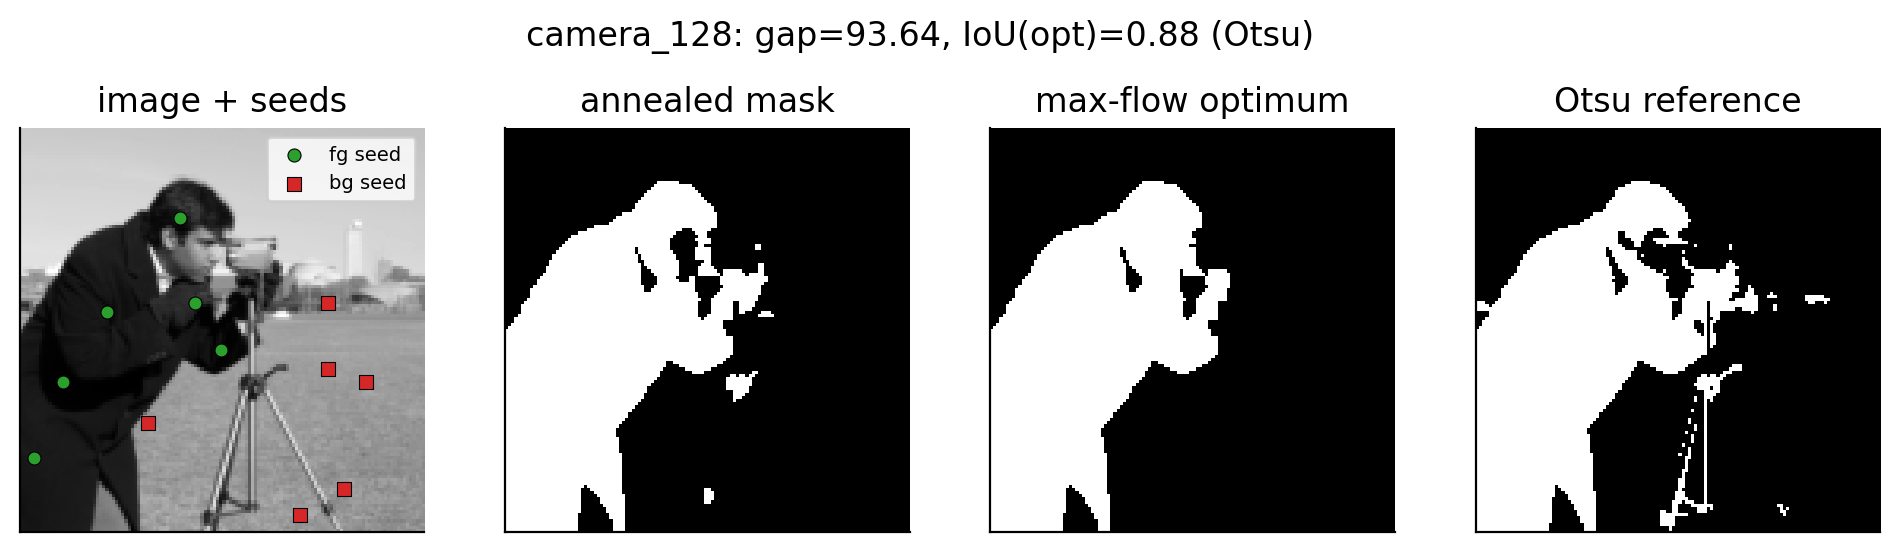
\includegraphics[width=0.95\linewidth]{../assets/seg_camera.png}\\[4pt]
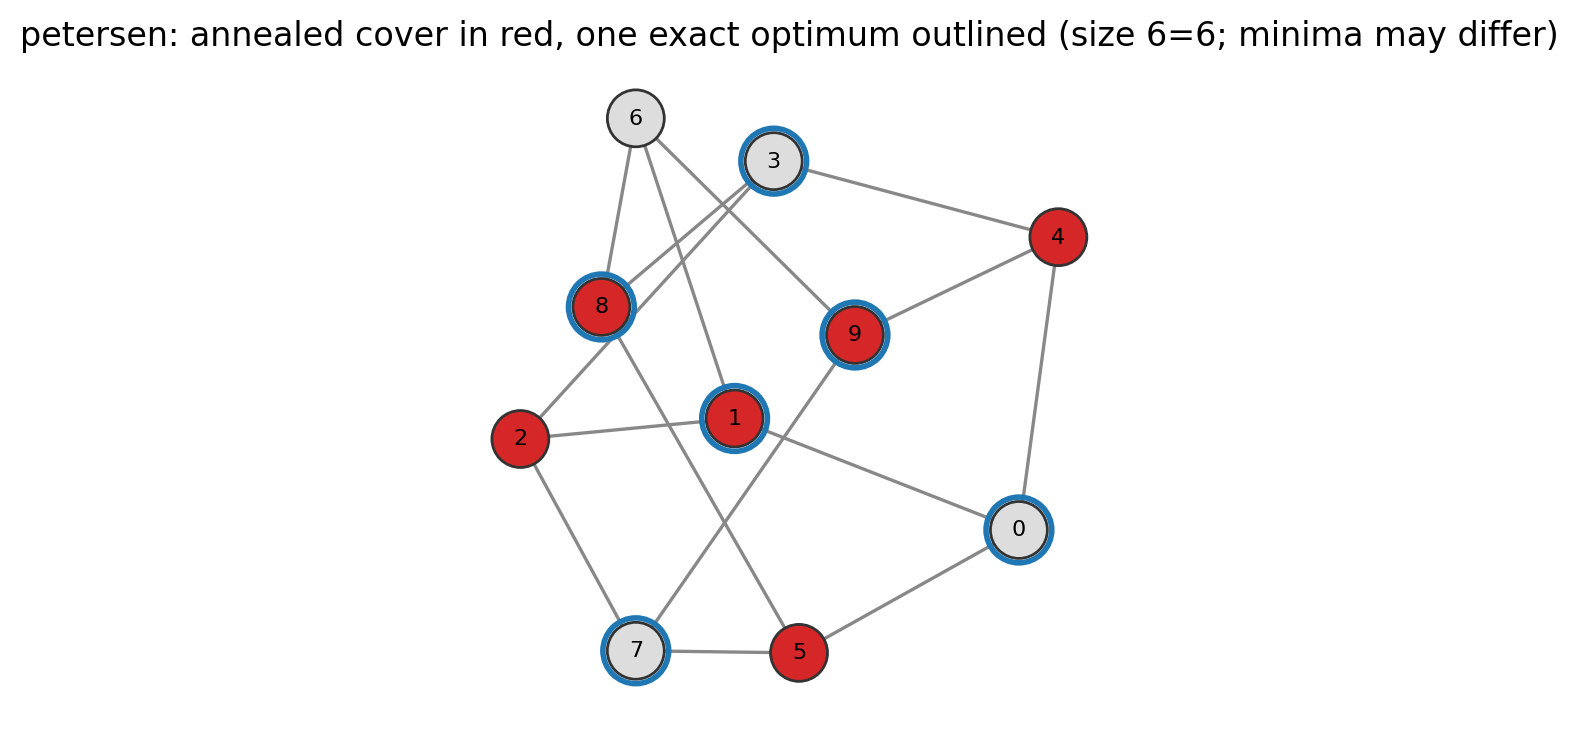
\includegraphics[width=0.46\linewidth]{../assets/vertex_cover.png}\hfill
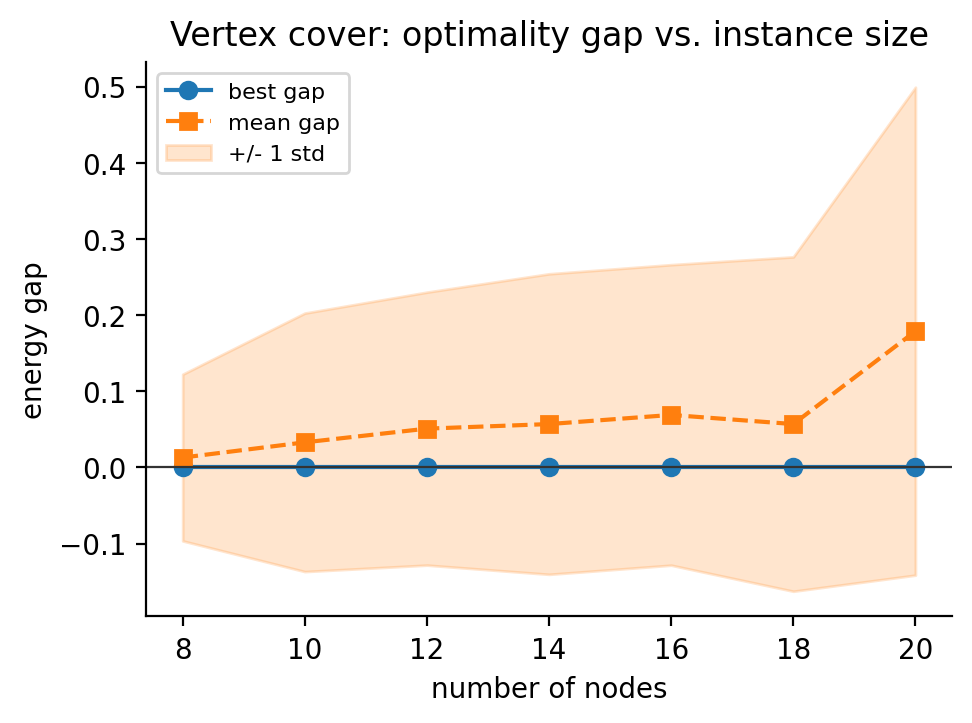
\includegraphics[width=0.50\linewidth]{../assets/gap_vs_size.png}
\caption{Top: high-resolution segmentation -- the annealed mask is identical to
the exact maximum-flow optimum and cleaner than an Otsu threshold. Bottom left:
a vertex-cover instance (annealed cover in red, one exact optimum outlined).
Bottom right: the optimality gap grows gently with instance size while the best
read stays optimal.}
\end{figure}

\paragraph{An integrity note.} The first real-image run produced \emph{negative}
optimality gaps (the heuristic appearing to beat the ``exact'' optimum), which
is impossible for a submodular energy. The cause was numerical: a large seed
penalty next to vanishingly small smoothness weights gave the floating-point
max-flow a $\sim\!10^{16}$ dynamic range, on which the solver returned a
non-minimum cut. Encoding seeds as \emph{bounded} infinities and using
integer-scaled capacities fixed it; gaps are now non-negative everywhere. An
exact reference is only as trustworthy as its numerics.

\section{New this update: a classical solver portfolio}
Following the methodology of Q-Seg~\cite{qseg} (which benchmarks against a
classical solver), we now run \emph{several} classical heuristics on the
identical QUBO and score each by its optimality gap to the exact reference and
its wall-clock time (Table~\ref{tab:portfolio}). Simulated annealing (SA), tabu
search, and steepest descent all consume the same \code{dimod} model.

\begin{table}[h]
\centering
\caption{Classical solver portfolio on the identical QUBO (100 reads). SA and
tabu reach the exact optimum on both problem classes; steepest descent
(``Greedy'') solves vertex cover but \textbf{fails on segmentation}, stalling in
local minima of the rugged labeling landscape.}
\label{tab:portfolio}
\small
\begin{tabular}{llrrrr}
\toprule
Problem & Solver & Mean gap & Max gap & Mean time (s) & Success \\
\midrule
Vertex cover & SA     & $0.000$  & $0.000$  & $0.013$ & $1.00$ \\
Vertex cover & Tabu   & $0.000$  & $0.000$  & $2.100$ & $1.00$ \\
Vertex cover & Greedy & $0.000$  & $0.000$  & $0.000$ & $1.00$ \\
Segmentation & SA     & $0.000$  & $0.000$  & $0.083$ & $1.00$ \\
Segmentation & Tabu   & $0.000$  & $0.000$  & $2.101$ & $1.00$ \\
Segmentation & Greedy & $13.20$  & $21.56$  & $0.002$ & $0.00$ \\
\bottomrule
\end{tabular}
\end{table}

\noindent The takeaway sharpens the project's message: the \emph{formulation} is
solver-agnostic, but the \emph{difficulty} is not. A trivial greedy descent
suffices for vertex cover yet is useless for segmentation, whereas SA and tabu
solve both -- a concrete, measured statement about which problems the QUBO move
makes easy or hard.

\section{Roadmap to increase effectiveness (no quantum hardware)}
The project's unique value is \emph{exactly validated, hand-designed
objectives}, not state-of-the-art segmentation. The most valuable improvements
therefore sharpen the solver comparison, add problems that retain an exact
check, and deepen the privacy bridge.
\begin{description}\itemsep2pt
  \item[Tier 1 (keeps exact validation).]
    (i) Extend the solver portfolio with parallel tempering and an exact MIP
    solver (Gurobi/OR-Tools) and report time-to-solution.
    (ii) Add a \emph{binary image denoising} phase (Greig et al.,
    1989~\cite{greig}): an Ising/MRF energy whose exact optimum is again a
    maximum-flow min-cut -- reinforcing the ``one objective, many problems''
    thesis nearly for free.
    (iii) GrabCut-style iterated graph cut to raise real-image IoU while staying
    hand-designed and exact per iteration.
    (iv) Statistical rigor: $\ge 10$ seeds, $95\%$ confidence intervals,
    time-to-target.
  \item[Tier 2 (research upside).]
    Deepen the GraphMI bridge -- reconstruct from a small trained GNN, and plot
    recovery F1 against feature noise and graph density (a privacy/utility
    curve), directly serving the lab's work on graph-data privacy. Add a
    Max-Cut / community-detection QUBO to fill out the ``graph partitioning''
    half of the title.
  \item[Tier 3 (scope expansion, trades the exact check).]
    Multi-label segmentation via $\alpha$-expansion; note that multiway cut is
    not submodular, so the clean max-flow reference is lost for $>2$ labels.
\end{description}

\section{Plan, reproducibility, and scope}
A day-by-day two-week schedule to a submittable final (report, poster, slides,
reproducibility harness, CI) is recorded in \code{docs/SCHEDULE.md}. The code is
public, tested, linted, and runs end-to-end on a laptop or via the included
Colab notebook; nothing requires quantum hardware. \textbf{Scope:} nothing is
learned from data; inputs are small and fixed-size so the exact reference stays
computable and the optimality gap remains the primary, interpretable measure of
success.

\begin{thebibliography}{9}
\bibitem{lucas} A.\ Lucas. \emph{Ising formulations of many NP problems.} Frontiers in Physics, 2014.
\bibitem{bj} Y.\ Boykov, M.-P.\ Jolly. \emph{Interactive graph cuts for optimal boundary \& region segmentation.} ICCV, 2001.
\bibitem{bk} Y.\ Boykov, V.\ Kolmogorov. \emph{An experimental comparison of min-cut/max-flow algorithms.} IEEE TPAMI, 2004.
\bibitem{greig} D.\ Greig, B.\ Porteous, A.\ Seheult. \emph{Exact maximum a posteriori estimation for binary images.} JRSS-B, 1989.
\bibitem{qseg} S.\,M.\ Venkatesh et al. \emph{Q-Seg: Quantum annealing-based unsupervised image segmentation.} arXiv:2311.12912, 2024.
\bibitem{graphmi} Z.\ Zhang et al. \emph{GraphMI: Extracting private graph data from graph neural networks.} IJCAI, 2021.
\end{thebibliography}

\end{document}
